% $File: application.tex
% $Date: Sat Jun 02 17:46:02 2012 +0800
% Author: Yuxin Wu <ppwwyyxxc@gmail.com>
\section{多项式方程组求解的实际应用}
\subsection{几何定理的机器证明}
	平面几何定理的机器证明,已有的有效方法主要有两种.
	一类是由张景中院士提出的基于面积的消点算法\cite{area_geo},
	一类是由吴文俊院士提出的基于代数方程的消元算法\cite{wwj},
	因为构造性平面几何命题的条件和结论可以表示为一系列次数不高的代数方程,
	因此代数方程组求解的理论对几何定理机器证明十分有用.
	
	如著名的Simson定理\footnote{详见\url{http://en.wikipedia.org/wiki/Simson_line}}:
	过$ P$点向$ \Delta ABC$三边做垂线,若$ P$在$ \Delta ABC$的外接圆上,则$  LMN$三点共线.
	\begin{figure}[h]
		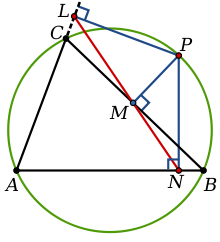
\includegraphics[width=10em]{res/Simson.png}
	\end{figure}

	以$ AB$中点为原点,$AB$方向为正方向,设$ A(-x_a,0),$ $B(x_a,0),$ $C(x_c,y_c),$ $P(x_p,y_p),$ $N(x_p,0),$ $M(x_m,y_m),$ $L(x_l,y_l)$.
	其条件可以化为如下代数方程组:
	\[  \begin{cases}
		PABC\texttt{共圆} &\Leftrightarrow y_cy_p^2-(y_c^2+x_c^2-x_a^2)y_p+y_c(x_p^2-x_a^2) =0\\
		PM\perp BC &\Leftrightarrow (x_c+x_a)(x_m-x_p)+y_c(y_m-y_p) =0\\
		M \in BC &\Leftrightarrow (x_c + x_a)y_n - y_c(x_n+x_a) =0\\
		PL \perp AC &\Leftrightarrow (x_c-x_a)(x_l-x_p) + y_c(y_l-y_p) = 0\\
		L \in AC &\Leftrightarrow (x_c-x_a)y_l - y_c(x_l-x_a)  = 0
	\end{cases}\]

	结论可写为: 
	$ (x_n-x_p)y_l - y_c(x_l-x_p) = 0$

	要证明原题结论,即证明上式在原方程组的生成理想中.
	吴文俊院士提出的机器证明方法,就是针对平面几何问题的特殊性提出的判断一多项式是否属于一个理想的快速方法.

\subsection{计算机图形学中的曲面拼接}
	在本学期选修的计算机系"计算机图形学基础"课程中,作者了解到多项式方程组求解在计算机几何造型的曲面拼接中的重要作用.

	对于一个参数曲面,传统的分析学中对连续性的定义不适用于图形学中
	,考虑参数方程表示的以下曲线\footnote{此例改编自胡事民老师"计算机图形学基础"课件}:
	\[  f(t) = \begin{cases} \dfrac{\overrightarrow X - \overrightarrow Y}{3}t,0\le t \le 1 \\
		\dfrac{\overrightarrow X - \overrightarrow Y}{3} + (t-1)\dfrac{2(\overrightarrow X - \overrightarrow Y)}{3},1 \le t \le 2
	\end{cases}\]

	参数连续性(Parametric Continuity)$ C^n $ 要求在各点的$ \dfrac{d^n f}{dt^n}$连续
	\footnote{详见\url{http://en.wikipedia.org/wiki/Smooth_function\#Parametric_continuity}}.
	在此例中,$ f'(1^-) \ne f'(1^+)$,因此在1处不满足$ C^1$连续,但事实上此函数图像为一直线.

	几何连续性(Geometric Continuity)$ G^n$忽略了参数在曲线上变化的速率,更适合描述图形学中的连续性.
	设$ P$点是曲面$ F_1 = 0, F_2 = 0$的一个公共点,
	若存在$ P$处非零的多项式$ A,B$使得$ AF_1-BF_2$的前$ k$阶导数均为0,则称两曲面在$ P$处$ G^k$连续.

	曲面拼接问题,就是对曲面$ F_1$与一辅助平面$ H=0$的交线$ C$,求曲面$ F_2$,使得$ F_2$与$ F_1$在$ C$上$ G^k$连续.
	其等价条件为, $ \exists \texttt{多项式}A,B,F_2 = AF + BH^{k+1}$,即$ F_2$在$ F_1$与$ H^{k+1}$的生成理想中\cite{warren}.
	因此这仍然是一个多项式代数的问题.
